
\documentclass[11pt, a4paper]{article}
\usepackage[left=4cm, right=4cm, %showframe
]{geometry}

%% \documentclass[paper=a4]{scrartcl}
%% \usepackage[left=4cm, right=4cm, %showframe
%% ]{geometry}

\usepackage{local_config}

\usepackage{titling}
\setlength{\droptitle}{-7em}

\usepackage{abstract}
\renewcommand{\abstractname}{}    % clear the title
\renewcommand{\absnamepos}{empty} % originally center

\usepackage{authblk}

\renewcommand\Affilfont{\fontsize{9}{10.8}\itshape}
%\renewcommand\Abstractfont{\fontsize{11pt}}

\title{Non-random network connectivity comes in pairs\vspace{-2ex}}
\date{}
\author[1,2,*]{Felix Z.~Hoffmann}
\author[1]{Jochen Triesch}

\affil[1]{Frankfurt Institute for Advanced Studies (FIAS), Johann Wolfgang Goethe University, Frankfurt am Main, Germany}
\affil[2]{International Max Planck Research School for Neural Circuits, Max Planck Institute for Brain Research, Frankfurt am Main, Germany\vspace{3ex}}
\affil[*]{Email: hoffmann@fias.uni-frankfurt.de\vspace{-13.5ex}}
\renewcommand\Authands{ and }


\begin{document}


%% \begin{center}
%% %{\Large{\textbf{ Non-random connectivity necessarily leads to an overrepresentation of bidirectional connections in networks with connection probablities that are symmetric in pairs}}}
%% {\Large{\textbf{ Non-random network connectivity comes in pairs }}}

%% %(connection probablities that are symmetric in pairs)
%% \end{center}
%% \centerline{}
%% \centerline{Felix Z.~Hoffmann, Jochen Triesch}


\maketitle
%
\begin{abstract}
Overrepresentation of bidirectional connections in local cortical networks has been repeatedly reported and has been in the focus of the discussion of non-random connectivity. Here we show in a brief mathematical analysis, that in a network in which connection probabilities are symmetric in pairs, $P_{ij} = P_{ji}$, the relative occurrence of bidirectional connections and non-random structures are inherently linked; an overabundance of reciprocally connected pairs emerges necessarily when the network structure deviates from a random network.
\end{abstract}
\vspace{0.2cm}


\section*{Introduction}

  %% Non-random network connectivity in a random graph can be modeled by assigning each connection a separate probability to exist. Some connections are more likely to be realized in the network, some less. In the limiting case a blue print. Here we assume a network with 

* connectivity is important for functional processes

* How does the brain establish these connections? Increasing evidence suggests that microcircuitry is highly non-random \cite{Song2005,Perin2011}. Thus not every connection is equally like established, rather some connections [...] If this process follows patterns in which both directions of connection within a pair are equally likely, we show that bidirectional connections are necessarily occurring more often than in a network in which each connection is equally likely.


* the story of bidirectional connections




\section*{Results}

  

%% Consider a network with nodes $x_1,\dots,x_{N}$. Let there be a connection from node $x_i$ to $x_j$ with probability $P_{ij}$. Typically, . However, it is highly unlikely that all nodes are connected with the same probability. 

%% Thus let the $P_{ij}$ be identically distributed continuous random variables with values in $[0,1]$. We write the of probability density function of the $P_{ij}$ as $f_{P_{ij}}$.


%% We're discussing now a network model in which node-to-node connection probabilities are randomly distributed. One might think for example of a network in which connection probability decreases with distance.

%% Remembering the notation from above, we write
%% \[
%% P(X_{ij}=1) = P_{ij}
%% \]
%% where $P=P_{ij}$ are identically distributed continuous random variables with values in $[0,1]$. We write the of probability density function of the $P_{ij}$ as $f_{P_{ij}}$.

The emergence of non-random connectivity patterns can be modeled by
assigning each possible connection in a random graph a separate
probability to exist.
%
In such a model some connections are more likely to be realized than
others, allowing for the encoding of patterns within the specific
probabilities of each connection.
%
In the limiting case each connection either exists or is absent with
certainty, representing a blueprint for the network architecture.
%

%
To analyze the effect of non-random structures within a network,
specifically on the statistics of bidirectionally connected pairs
found in the network, we consider a random graph model of $N$ neurons
in which the probability of node $i$ to connect to node $j$ is modeled by a random variable $P_{ij}$.
%
For this we assume $P_{ij}$ for $i,j = 1,\dots,N$ with $i \neq j$ to be
identically distributed random variables in $[0,1]$, yielding a
probability of connection for each ordered pair of nodes in the graph.
%
Outside of pairs the random variables $P_{ij}$ are assumed to be independent, that is non-equal $P_{ij}$ and $P_{kl}$ are independent as long as $i \neq l$ or $j \neq k$.
%
Finally, we explicitly exclude self-connections in this model and assume at all
times that $i \neq j$.% Below we're assuming $i \neq j $ in all cases.
% where we
%always assume $i \neq as it does not make sense to consider
%bidirectional connectivity in
%% self-connections.
%

%
Given the distributions of connection probabilities, what is
then the probability in this model for a randomly selected node to have a
projection to another randomly selected node?
%
As the random variables $P_{ij}$ are identically distributed, we
compute this overall connection probability $\mu$ easily as the
expected value of~$P_{ij}$,
\begin{align}
\mu = \E(P_{ij}).
\end{align}
%
For example, if the $P_{ij}$ have a probability density function $f$ with essential support in $[0,1]$, we can compute the connection fraction as
\begin{align}
  \mu = \int_0^1 x f(x)\,dx.
\end{align}

In this work we are interested in the probability $P_{\mathbf{bidir}}$
of a bidirectional connection to exist in a random pair of neurons.
%
We determine $P_{\mathbf{bidir}}$ as the expected value of the product
of $P_{ij}$ and $P_{ji}$,
%
\begin{align}
P_{\mathbf{bidir}} = \E(P_{ij} P_{ji}).
\end{align}
%
The relative occurrence $\varrho$ of such reciprocally connected pairs compares $P_{\mathbf{bidir}}$ with the occurrence of bidirectional pairs in an Erd\H{o}s-R\'{e}nyi graph, in which each unidirectional connection is equally likely to occur with probability $\mu$ \cite{Gilbert1959, Erdos1959}. The probability of a particular bidirectional connection to exist in such a random graph is simply $\mu^2$ and we obtain the relative occurrence as the quotient
%% To answer the question if this probability is deviates from the proabibility than we would expect . The probability of a bidirectional in this standard random graph is $\mu$. We can the overrepresentation of as the quotient of $
\begin{align}
\varrho = \frac{P_{\mathbf{bidir}}}{\mu^2} = \frac{\E(P_{ij}P_{ji})}{{\E\left(P_{ij}\right)}^2}.\label{eq:rho}
\end{align}
%
Experimental studies in local cortical circuits of rodents have repeatedly reported a relative occurrence of bidirectional connections $\varrho > 1$ \cite{Markram1997, Song2005, Perin2011}. To understand in which cases such an overrepresentation occurs, we consider two cases. In the first case, assume now that connection probabilities are independently determined in pairs as well, meaning that the random variables $P_{ij}$ and $P_{ji}$ are independent. Then, as $P_{ij}$ and $P_{ji}$ are identically distributed,
\begin{align}
\E(P_{ij} P_{ji}) = \E(P_{ij})\,\E(P_{ji}) = \E(P_{ij})^2,
\end{align}
and we expect to observe no overrepresentation of reciprocal connections, $\varrho = 1$.  In the second case, assume then that connection probabilities are symmetric in pairs, $P_{ij} = P_{ji}$. In this case,
\begin{align}
P_{\mathbf{bidir}} = \E(P_{ij}^2),
\end{align}
%
and the expected relative occurrence of reciprocal connections becomes
\begin{align}
\varrho = \frac{\E(P_{ij}^2)}{{\E\left(P_{ij}\right)}^2}.
\end{align}
We note that now any distribution of $P_{ij}$ with a nonvanishing
variance will lead to a relative occurrence that deviates from the
Erd\H{o}s-R\'{e}nyi graph, as
\begin{align}
\Var(P_{ij}) = \E(P_{ij}^2) - \E\left(P_{ij}\right)^2.
\end{align}
Moreover, since $x \mapsto x^2$ is a strictly convex function, Jensen's inequality \cite{Jensen1906, Cover2006} yields
\begin{align}
\E(P_{ij}^2) \geq \E(P_{ij})^2, \label{eq:jensen}
\end{align}
and we find that $\varrho \geq 1$ in networks with symmetric connection probabilities. Jensen's inequality further states that equality in \eqref{eq:jensen}, and thus $\varrho = 1$, holds if and only if $P_{ij}$ follows a degenerate distribution, that is if all $P_{ij}$ take the identical value $\mu$. In the other case, where the $P_{ij}$ take on more than one value with non-zero probability, we speak of a non-degenerate distribution.

As a central result of this study we thus find that any non-degenerate distribution of symmetric connection probabilities ($P_{ij} = P_{ji}$) necessarily induces an overrepresentation of bidirectional connections in the network, $\varrho > 1$. In other words, in a network in which both directions of connection are equally likely within any given pair, but where some pairs are more likely to be connected than others, the count of expected reciprocally connected pairs is strictly underestimated by the statistics of an Erd\H{o}s-R\'{e}nyi graph with same the overall connection probability $\E(P_{ij}) = \mu$.

%connections are more likely to exist in some pairs than in others, 

%% ensuring an overrepresentation of bidirectional connections $\varrho > 1$ for any non-degenerate distribution of connection probabilities in the network. In other words, in a network model where some pairs are more likely connected than others, the count of expected reciprocally connected pairs is strictly underestimated by the statistics of an Erd\H{o}s-R\'{e}nyi graph with same overall connection probability $\E(P_{ij}) = \mu$.



%% Finally we can write the expected overrepresentation as
%% \[
%% \varrho = \frac{\E(P_{ij}^2)}{{\E\left(P_{ij}\right)}^2}.
%% \]




  \subsection*{Upper bound for $\varrho$}

    
The overrepresentation of bidirectional connections $\varrho$ in a network is maximal when every connected pair is already a reciprocally connected pair. In terms of the model defined above, this is the case when
\begin{align}
\E(P_{ij} P_{ji}) = \E(P_{ij}).
\end{align}
%
The relative occurrence of reciprocal connections from \eqref{eq:rho} then becomes
\begin{align}
\varrho = \frac{1}{\E(P_{ij})} = \frac{1}{\mu} \label{eq:rho_max}
\end{align}
Thus, for local cortical circuits of L5 pyramidal neurons with a typical connection probability of $\mu = 0.1$ \cite{Thomson2002,Song2005}, the network model yields a maximal overrepresentation of $\varrho = 10$. While this theoretical maximum is unlikely to exist in actual cortical networks, the precise degree of overrepresentation will depend on the specific distribution of connection probabilities in the network. In the following, we study two generic examples.


  \subsection*{Two-point distribution}  

    
The simplest non-constant distribution of connection probabilities is a distribution that takes two values $x$, $y$ with probability $p$ and $1-p$ respectively. Formally, let $0 \leq x,y \leq 1$ with $x \neq y$  and $0 < p < 1$. Then a random variable $X$ follows the two-point distribution %% \cc{(\enquote{Zweitpunktverteilung}, \href{https://de.wikipedia.org/wiki/Zweipunktverteilung}{Wiki})}
$\mathcal{T}(p,x,y)$ if $P(X=x)=p$ and $P(X=y) = 1-p$. 

In our network model let then the $P_{ij}$ be $\mathcal{T}(p,x,y)$ distributed. The overall connection probability $\mu$ is
\begin{align}
\mu = \E(P_{ij}) = px + (1-p)y. \label{eq:bd1}
\end{align}
%% Given $\mu$,$x$ and $y$, the probability $p$ calculates as
%% \begin{align}
%%   p = \frac{c-y}{x-y}. \label{eq:bd1}
%% \end{align}
Assume again that $P_{ij} = P_{ji}$. The relative occurrence of bidirectional connections is given by
\begin{align}
  \sigma = \frac{\E(P_{ij}^2)}{\mu^2} = \frac{p x^2 + (1-p) y^2}{\mu^2} \label{eq:bd2}
\end{align}
Solving \eqref{eq:bd1} for $p$ and inserting into equation~\eqref{eq:bd2} yields an expression for the relative overrepresentation depending on $x$, $y$ and $\mu$ (see Appendix),
\begin{align}
\sigma = \frac{x+y}{\mu} - \frac{xy}{\mu^2}.
\end{align}

\begin{figure}[h!]
\centering
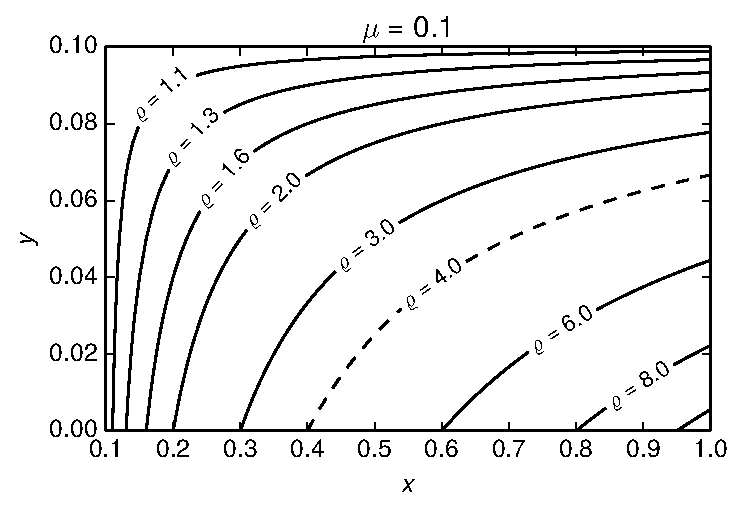
\includegraphics[width=0.65\textwidth]{../lab/two_point_distribution/contour_plot.png}
\caption{Contour plot shows the relative overrepresentation $\sigma$ obtained from different pairings of $x$ and $y$ for two-point distributed connection probabilities, $P_{ij} \sim \mathcal{T}(\frac{\mu-y}{x-y},x,y)$ with $\mu = 0.1$. The dashed line marks an overrepresentation of bidirectional connections of $\sigma=4$ as observed by \textcite{Song2005} in their experimental study.}
\label{fig:tp}
\end{figure}

In local cortical circuits, a single neuron is typically projecting to roughly 10\% of the population. Fixing $\mu = 0.1$, we obtain the relative occurrence dependent on the two connection probability values $x$ and $y$. Without restriction we can assume $x \geq \mu$ and it follows that $y \leq \mu$ (see Appendix). Possible values for $x$ and $y$ are then $0.1 \leq x \leq 1$ and $0 \leq y \leq 0.1$. Figure~\ref{fig:tp} shows contours of $\sigma$ for the $(x,y)$ pairings illustrating how different values for the relative overrepresentation of reciprocal connections can be induced by two-point distributed connection probabilities.  







  \subsection*{Gamma distribution}

    
A continuous distribution  long tail and narrow while maintaing a constant mean. The gamma distribution fulfills these criteria.

Here we consider a slight modification to the traditional Gamma distribution in the form of a truncated version. Let $\alpha, \beta > 0$. A random variable $X$ follows the truncated gamma distribution $\Gamma^T(\alpha, \beta)$ if it has the probability density function 
%
\begin{align}
  f_{\alpha,\beta}(x) = \begin{cases} K_{\alpha, \beta}\,
\frac{1}{\beta^{\alpha}\Gamma(\alpha)}\, x^{\alpha-1}\,e^{-x/\beta} & 0 \leq x \leq 1 \\
0 & \text{otherwise}.
\end{cases}
\end{align}
%
Here the factor $K_{\alpha,\beta}$ is needed due to the truncation of the probability density function for $x>0$ to ensure that
\begin{align}
  \int f_{\alpha,\beta}(x) \,dx = 1. \label{eq:gd1}
\end{align}
The value of $K_{\alpha,\beta}$ is the inverse of the cumulative probability $x \leq 1$ of the untruncated gamma distribution,
\begin{align}
  K_{\alpha,\beta} = \left(\int_0^{1} \frac{1}{\beta^{\alpha}\Gamma(\alpha)}\, x^{\alpha-1}\,e^{-x/\beta} \, dx \right)^{-1}.
\end{align}
With this the equality~\eqref{eq:gd1} clearly holds. Consider then the above network model in which the connection probabilities $P_{ij}$ are $\Gamma^T(\alpha, \beta)$ distributed. As $K_{\alpha,\beta}$ is results hold. We note the following results for the overall connection probability $\mu$,

\begin{align}
 \mu = \E(P_{ij}) = K_{\alpha,\beta} \, \alpha \beta,
\end{align}
and the expected occurrence of bidirectional connections
\begin{align}
  \E(P_{ij}^2) = K_{\alpha,\beta}^2 \, (\alpha^2 \beta^2 + \alpha \beta^2).
\end{align}

The overrepresentation is then
\begin{align}
  \sigma & = \frac{\E(P_{ij}^2)}{\E(P_{ij})^2} =% \frac{\alpha^2 \beta^2}{\alpha^2 \beta^2} + \frac{\alpha \beta^2}{\alpha^2 \beta^2} =
  1 + \frac{1}{\alpha}.
\end{align}


\begin{figure}[h!]
\centering
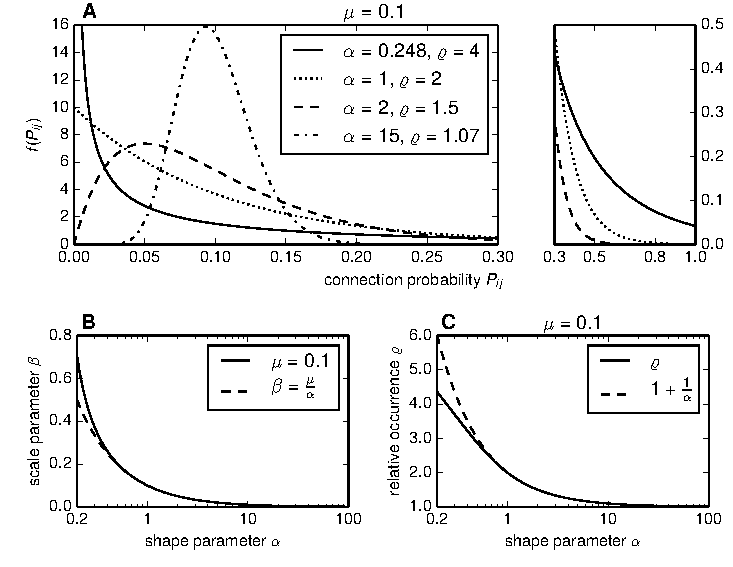
\includegraphics[width=\textwidth]{../lab/gamma_distribution/gamma_figure.png}
\caption{Probability density functions of the truncated gamma distribution for different shape parameters $\alpha$ and the induced relative overrepresentation of bidirectional connections $\sigma$ in the network. Note that only showing the distribution for values up to 0.5. For given $\alpha$ the parameter $\beta$ was estimated numerically to yield $\mu \approx 0.1$ in all distributions shown.}
\end{figure}


References: \href{http://herbsusmann.com/distributions/gamma-distribution-variance-proof.html}{Proof $\E(X^2)$}, 



     
\section*{Discussion}


We were able to show that a relative overrepresentation of bidirectional connections arrises necessarily in networks with a non-degenerate distribution of symmetric connection probabilities. Conversely, an absence of an overabundance of reciprocal pairs, as for example found in the intra-layer connectivity of the mouse C2 barrel column \cite{Lefort2009}, points towards either a truly random network or an asymmetry in the connection probabilities. 

Quantitatively, a network in which connection probabilities take on one of two values is easily able to account for even the highest values of overrepresentation reported. A network with such a two-point distribution of connection probabilities is likely two occur naturally, where the connection probability depends on whether a given pair of neurons shares a certain feature, such as a common orientation preference \cite{Lee2016}, or not. 

A continuous distribution in connection probabilities on the other hand might occur when pair connectivity depends on a continuous parameter such as the distance between neurons, the neurons' age or intrinsic parameters of connectivity. We showed that networks in which connection probabilities follow a gamma distribution can as well have a high relative occurrence of reciprocally connected pairs, however in this case a larger fraction of pairs remains almost certainly unconnected.

It is likely that a combination of both the discrete and continuous effects determines the connection probabilities in local cortical networks. We showed that as long as this probability is symmetric for pairs, any effect on .

When reciprocal pairs are absent, One could argue that neither distance-dependency nor functionally specific . As we have no reason to believe, might in fact be so small that no . Following this logic, we predict that no prevalent feature that by itself can predict as we would in this case, assuming symmetric connection probabilities, expect to see an overrepresentation of bidirectional connections.


%% * What are mechanisms that could affect connection probabilities in a symmetric manner? $\rightarrow$ Distance-dependency (Song vs. Perin), ...

%% * What are mechanisms that favor a certain direction of connection? $\rightarrow$ Morphology, ...

* Conclusion: Overrepresentation of bidirectional emerges as a \enquote{symptom} of \textbf{any} non-random connectivity $+$ symmetric connectivity, thus not necessarily an intrinsic parameter of network connectivity

* Research question should thus possibly focus more on 1) higher order non-random structures or 2) weights of connectivity (example: bidirectionally connected pairs typically have strong weights). 


* Why this is an important result: Overrepresentation of bidirectional connections maybe more a symptom of non-randomness + symmetry. Insight allows the formulation of possibly more important questions (weights of bidirectional connections etc..)



\newpage
\section*{Supplementary Material}
The supplementary information document for references SI1 and SI2 is available online at \textsc{doi}:~\texttt{\href{https://dx.doi.org/10.6084/m9.figshare.3501860}{10.6084/m9.figshare.3501860}}. Python code for the numerical computations is available as a GitHub repository and was archived at \textsc{doi}:~\texttt{\href{http://doi.org/10.5281/zenodo.154007}{10.5281/zenodo.154007}}. A website documenting the code is found at \texttt{\href{https://non-random-connectivity-comes-in-pairs.github.io/}{https://non-random-connectivity-comes-in-pairs.github.io/}}.

\section*{Acknowledgements}
JT is supported by the Quandt foundation.


  
%\section{Appendix}

% \subsection{Two-point distribution}

Solving \eqref{eq:bd1} for $p$ gives
\begin{align}
  p = \frac{\mu-y}{x-y},
\end{align}
%
which, plugged into \eqref{eq:bd2}, yields
\begin{align}
  \varrho & = \frac{\left(\frac{\mu-y}{x-y}\right)x^2  + \left(1-\frac{\mu-y}{x-y}\right) y^2}{\mu^2} \\ & = \underbrace{\frac{(\mu - y)x^2}{(x-y)\mu^2}}_{\mathrm{(I)}}\,\, + \,\, \underbrace{\frac{y^2}{\mu^2}}_{\mathrm{(II)}}\,\, - \,\, \underbrace{\frac{(\mu - y)y^2}{(x-y) \mu^2}}_{\mathrm{(III)}}.
\end{align}

The summands are
\begin{align}
  \mathrm{(I):} \quad & \frac{(\mu - y)x^2}{(x-y)\mu^2} = \frac{x^2}{(x-y)\mu} - \frac{yx^2}{(x-y)\mu^2} \\
  \mathrm{(II):} \quad &  \frac{y^2}{\mu^2} = \frac{(x-y)y^2}{(x-y)\mu^2} = \frac{xy^2}{(x-y)\mu^2} - \frac{y^3}{(x-y)\mu^2} \\
  \mathrm{(III):} \quad & - \frac{(\mu - y)y^2}{(x-y) \mu^2} = \frac{y^3}{(x-y)\mu^2} - \frac{y^2}{(x-y)\mu}
\end{align}

Putting everything together we get
\begin{align}
  \varrho & =  \frac{x^2 - y^2}{(x-y)\mu} + \frac{xy^2 -yx^2}{(x-y)\mu^2}  = \frac{(x + y) (x-y)}{(x-y)\mu} - \frac{xy (x-y)}{(x-y)\mu^2} \\
  & = \frac{x+y}{\mu} - \frac{xy}{\mu^2}.
\end{align}

------------------------------------------------------------------------------------------------------

Given $x \geq \mu$. From \eqref{eq:bd1} we have
\begin{align}
  y = \frac{\mu - px}{1-p} \leq \frac{(1-p)x}{1-p} = x.
\end{align}

Assume then $y > x$. It follows that
\begin{align}
  \mu < y = py + (1-p)y \leq px + (1-p)y = \mu
\end{align}
yielding a contradiction. Thus $y \leq \mu$.


%% See aslo: \href{https://www.wolframalpha.com/input/?i=Simplify[%28%28%28c-y%29%2F%28x-y%29%29*x^2%2B%281-%28%28c-y%29%2F%28x-y%29%29%29*y^2%29%2Fc^2]}{Wolfram Alpha}.


%\clearpage

\printbibliography
  
  
\end{document}


